\documentclass[conference]{IEEEtran}
\IEEEoverridecommandlockouts
\usepackage{cite}
\usepackage{amsmath,amssymb,amsfonts}
\usepackage{algorithmic}
\usepackage{graphicx}
\usepackage{textcomp}
\usepackage{xcolor}
\def\BibTeX{{\rm B\kern-.05em{\sc i\kern-.025em b}\kern-.08em
    T\kern-.1667em\lower.7ex\hbox{E}\kern-.125emX}}

\begin{document}

% Header
\title{RISKVI Case Study\\}
\author{\IEEEauthorblockN{Jonathan Wang}
\IEEEauthorblockA{\textit{Electrical and Computer Engineering} \\
\textit{University of Utah}\\
Salt Lake City, Utah \\
u1306458@umail.utah.edu}
}
\maketitle

% Abstract
\begin{abstract}
RISK-V FPGAs are attracting chip developers worldwide due to their open source and 
ease of configuration. These FPGAs can be used in space applications. Implementing fast and reliable 
hardware on nanosatellites had to be tested under extreme circumstances. This report evaluates the
impact of the operating system on the reliability of RISC-V based FPGAs against configuration
memory upsets. 
\end{abstract}
\begin{IEEEkeywords}
RISC-V, FPGAs, nanosatellites, configuration memory upsets
\end{IEEEkeywords}

% Introduction
\section{Introduction}
Field-programmable gate arrays(FPGAs) are becoming attractive for nanosats due to the improvements in 
performance and in-field reconfigurability of new generations of SRAM-based FPGAs. A nanosat or nanosatellite(Fig. 1)
is anything that weighs between 1 and 10 kilograms. They are becoming attractive for space travel due to improvements 
in performance and in-field reconfigurability compared to traditional computer chips.
The software running on the FPGAs is called Embedded Operating System. An Embedded OS is a specialized operating system
designed to perform a specific task for a device that is not a computer. The main job of an embedded OS is to run the 
code that allows the device to do its job, and it makes software development easier. 
\begin{figure}[h]
    \centering
    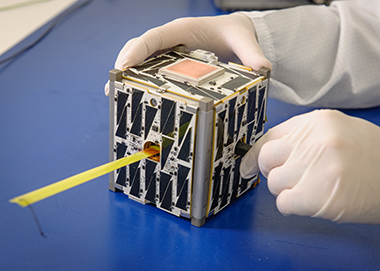
\includegraphics[scale = 2.5]{nanosat.jpg}
    \caption{A real life nanosat.}
\end{figure}
Current operating systems that are qualified for space missions are generally very costly. Consequently, general-purpose
OS-powered nanosat missions, such as Linux systems, have been deployed in the past. Leppinen \cite{b1} stated that choosing 
Linux limits the choice of hardware. Another major drawback is that Linux is not designed to be a real-time operating 
system. A real-time operating system is an OS that guarantees real-time applications a certain capability within a specified 
deadline. In some cases, design changes can reduce the number of hard real-time applications. The remaining constraints 
require another dedicated controller to handle the real-time problem. 

% Background clarification
\section{Background}
The reliability of these OSs for a given hardware platform needs to be evaluated before their actual deployment.
Wali et al. \cite{b2} assessed the effects of the Linux OS on the fault tolerance of applications running on a RISC-V 
SoC(System on Chip) implemented in a Xilinx FPGA. To address the evaluation of the effects, we need to define the 
background. Although previous studies analyzed the fault tolerance of OS in embedded platforms, the following 
report will focus on radiation-induced configuration memory upsets on the reliability of applications running on 
a Linux RISC-V FPGA. Radiation-induced configuration memory upsets are a type of computer hardware failure caused 
by exposure to ionizing radiation from space. The radiation can create a charge that alters the state of a memory 
cell, causing a bit flip when the chip is exposed. It can result in errors in data storage or retrieval. In some
cases, it can crash the system. 
\subsection{FPGA Fault Injection} % Injection method
The method employed is called FPGA fault injection. It is defined as the validation technique of fault-tolerant 
systems where the observation of the system's behavior in presence of faults is done explicitly by 
injecting faults into the system. Reference \cite{b2} pointed out that FPGAs are an ideal fault-emulation platform 
due to their high logic density and reconfigurability. The FPGA consists of two layers, the user layer, and the configuration 
layer. Partially Modifying the configuration layer can start the injection process. Tawfeek et al. categorized the fault 
injection technique into three categories in \cite{b4}. In our case, we will be using software-based injection. 
The objective is to inject errors at the software level. The injected error simulates those that may occur due to hardware faults. 

% Experiment details
\section{Experiment Setup and Overview}
The hardware the experiment uses includes an Artix-7 series FPGA from Xilinx Inc. and a host computer. 
\subsection{Hardware Setup}
Figure 2 shows the block diagram of the hardware setup. 
The host computer is responsible for the fault injections and the debug software, which communicates with the FPGA's SoC
through a debug interface. The interface controls the executions of workload programs, collection of data, logging the errors,
and resets the program for the following execution.  
\begin{figure}[h]
    \centering
    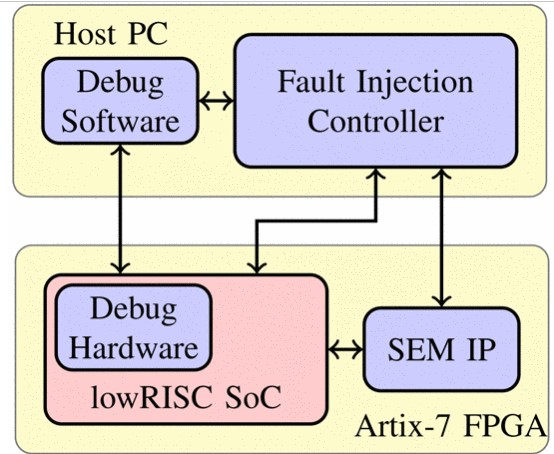
\includegraphics[scale = 0.5]{fault_inject.jpg}
    \caption{Block diagram of the fault injection setup.}
\end{figure}
The fault injection controller is located inside the host computer and utilizes Soft Error Mitigation Intellectual Property (SEM IP)
to introduce single event upsets (SEUs) into the Artix-7 FPGA's configuration memory. Maillard et al. from Xilinx performed 
a similar analysis\cite{b3} to simulate the impact of radiation on the FPGA, but they utilized a proton beam rather than actual radiation.





% Citations
\begin{thebibliography}{10}
    \bibitem{b1} H. Leppinen, "Current use of linux in spacecraft flight software," in IEEE Aerospace and Electronic Systems Magazine,
     vol. 32, no. 10, pp. 4-13, October 2017, doi: 10.1109/MAES.2017.160182. 
    \bibitem{b2} I. Wali, A. Sánchez-Macián, A. Ramos and J. A. Maestro, "Analyzing the impact of the Operating System on the Reliability
     of a RISC-V FPGA Implementation," 2020 27th IEEE International Conference on Electronics, Circuits and Systems (ICECS), Glasgow, UK, 2020,
    pp. 1-4, doi: 10.1109/ICECS49266.2020.9294858.
    \bibitem{b3} P. Maillard et al., "Single-Event Evaluation of Xilinx 16nm UltraScale+™ Single Event Mitigation IP," 2018 IEEE Radiation 
     Effects Data Workshop (REDW), Waikoloa, HI, USA, 2018, pp. 1-5, doi: 10.1109/NSREC.2018.8584298.
    \bibitem{b4} R. M. Tawfeek, M. G. Egila, Y. Alkabani and I. M. Hafez, "Fault injection for FPGA applications in the space," 2017 12th
     International Conference on Computer Engineering and Systems (ICCES), Cairo, Egypt, 2017, pp. 390-395, doi: 10.1109/ICCES.2017.8275338.
     
    
\end{thebibliography}

\end{document}
